\section{Machine Learning Models}
\label{sec:ML}
As price prediction is a common regression task, multiple regressors are trained separately. The best-performing 
models are then ensembled using a \textbf{VotingRegressor} to achieve the best possible performance.

\subsection{Regression Models}
\label{sec:regression_models}
For the single regressor models, the models \textit{XGBoost} (one tree-based and one based on linear models), \textit{CatBoost},
\textit{AdaBoost} and \textit{ExtraTrees} are trained and compared using the three scaling methods discussed in \autoref{sec:Expl}
and also compared to no scaling.\\
The target variable \textit{Price} is transformed by a logarithmic function. Models based on a Min-Max scaling of the price yielded on worse results
on average. To split the data into training and testing subsets, the train-test split function of the sklearn.modelselection
library is used with a ration of  $30 \, \% $ for testing and $ 70 \, \%$ for training.\\
For the training of the individual models, a Pipeline comprising a \textit{preprocessor}, \textit{feature selection} and the 
respective \textit{regressor} is deployed. The preprocessor includes a numeric and categorical transformer. The numeric preprocessor uses 
a SimpleImputer to fill missing entries with the mean and scales entries according to the chosen scaling method. The categorical
preprocessor uses a SimpleImputer to fill \texttt{NaNs} with the most frequent entry value and handles categorical values
with a OneHotEncoder, creating dummy columns. For the CatBoost model, no categorical transformation is applied, as one of the strengths
of this model is the handling of categorical data.\\
The feature selection is carried out using an Extra Trees Regressor, to evaluate the most important features, which are then used 
for the training. For the CatBoost model, no feature selection is performed, due to challenges with transformating
the categorical data. Hyperparameters are optimised using a \textbf{RandomizedSearchCV} grid search with 10-fold cross validation. The best parameters
for each model's scaling can be found in the \autoref{sec:Appendix}.\\
To evaluate the model performance a 10-fold Cross-Validation of the Root Mean Squared Error (RMSE) is performed and the Mean Squared Error (MSE),
Mean Absolute Error (MAE), $ \mathrm{R}^2 $ are extracted using the test subset and the Training Time (TT) is recorded. The results for the best-performing models
are displayed in \autoref{tab:Metrics}. The full table can be found in the \autoref{sec:Appendix}. The best models are chosen based on their $R^2$ score, MAE and the standard deviation of the RMSE.
The $R^2$ score indicated how well the true prices can be explained by the regression, with values ranging from $0$ to $1$.
The MSE on the other hand, measures the average squared difference between predicted and true values, penalizing large residuals.
The MAE measures the average absolute error of the predicted data points.
In this use case, the $R^2$ - score and MAE are chosen as the main metrics to compare the different data models. Large residuals usually
arise from motorcycles that are limited in quantity or are of particularly bad quality and therefore sell way below or above the market value.
Since this information is not included in the training of the model, these entries result in high MSE. Therefore, the MAE appears to 
be the more effective measure to quantify errors. 
\begin{table}[h!]
    \centering
      \begin{tabular}{ |p{2cm}||p{2cm}||p{2.9cm}|p{1.9cm}|p{1.7cm}|p{1cm}|p{1.2cm}|  }
        \hline
        \multicolumn{7}{|c|}{Evaluation Individual Regressors} \\
        \hline
        Model & Scaler & RMSE / €  & MSE / €  & MAE / € & $ \mathrm{R}^2 $& TT / s\\
        \hline
        \multirow{4}{2cm}{XGBoost (Tree)} & Standard & $2400.5 \pm  429.7$ & $4557951.9$ & $1350.6$ & $0.894$ & $2.37$\\
        & \cellcolor[HTML]{FFFACD} Gaussian  & \cellcolor[HTML]{FFFACD} $2379.3 \pm  395.6$ & $4514569.4$ & \cellcolor[HTML]{FFFACD} $1352.1$ & \cellcolor[HTML]{FFFACD} $0.897$ & $2.42$\\
        & Robust & $2405.0 \pm  425.2$ & $4500529.4$ & $1356.1$ & $0.895$ & $2.71$\\
        & No Scaling & $2389.3 \pm  415.9$ & $4479635.3$ & $1342.4$ & $0.897$ & $2.35$\\
        \hline   
        \multirow{4}{2cm}{CatBoost} & \cellcolor[HTML]{98FB98} Standard & \cellcolor[HTML]{FFFACD} $2334.1 \pm  386.9$ & $4146873.1$ & \cellcolor[HTML]{FFFACD} $1297.3$ & \cellcolor[HTML]{FFFACD} $0.902$ & $2.15$\\
        & Gaussian  & $3460.8 \pm  500.0$ & $4407888.2$ & $1320.6$ & $0.899$ & $1.73$\\
        & Robust & $2343.9 \pm 395.1$ & $4174227.2$ & $1305.9$ & $0.899$ & $2.51$\\
        & No Scaling & $2310.0 \pm  417.6$ & $4148775.5$ & $1300.4$ & $0.901$ & $1.81$\\
        \hline   
        \multirow{4}{2cm}{Extra Trees} & Standard & $2494.6 \pm  407.3$ & $4481129.5$ & $1349.5$ & $0.889$ & $3.47$\\
        & Gaussian  & $2507.0 \pm  391.9$ & $4426545.2$ & $1357.3$ & $0.886$ & $3.47$\\
        & \cellcolor[HTML]{FFFACD} Robust & \cellcolor[HTML]{FFFACD} $2470.0 \pm 408.5$ & $4394657.3$ & \cellcolor[HTML]{FFFACD}$1339.0$ & \cellcolor[HTML]{FFFACD}$0.890$ & $3.76$\\
        & No Scaling & $2517.8 \pm  435.9$ & $4590153.2$ & $1369.7$ & $0.891$ & $3.94$\\
        \hline
      \end{tabular}
      \caption{RMSE, MSE, MAE, $R^2$ score and training time for the best performing individual models and applied scaling methods. The best-performing values are highlighted.}
      \label{tab:Metrics}
\end{table}
The most important attributes chosen by feature selection with the ExtraTrees Regressor and the different scaling methods applied are 
visually presented in the \autoref{sec:Appendix}.\\
According to the training with optimised hyperparameters, the \textbf{tree-based XGBoost} model with
\textbf{gaussian} scaling, the \textbf{CatBoost} model with \textbf{standard} scaling and the \textbf{Extra Trees} model with \textbf{robust} scaling are performing best and are
chosen for the ensembled model.

\subsection{Ensembled Model}

To create an ensembled model of the best-performing models, a VotingRegressor is used. The weights of the individual models
for the VotingRegressor are determined through hyperparameter optimisation using a RandomizedSearchCV grid search. The optimal weights 
are $2:1:1$ corresponding to CatBoost:ExtraTrees:XGBoost, respectively.
A schematic visual representation of the ensembled model pipeline is shown in \autoref{fig:EnsembledModel}.
\begin{figure}
    \centering
        \makebox[\textwidth][c]{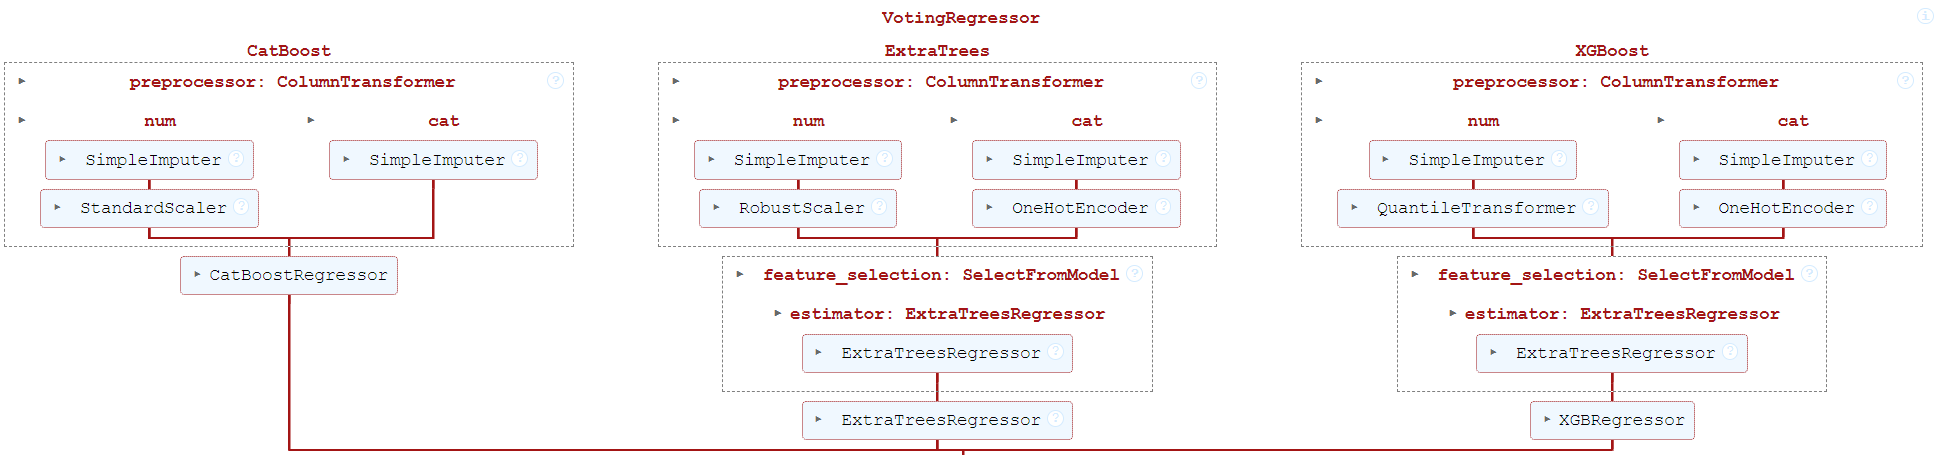
\includegraphics[width=1.25\textwidth]{"content/pics/Ensembled_Model_compromised.png"}}
        \caption{Schematic view of the ensembled model showing the single pipeline steps (preprocessing and feature selection).}
        \label{fig:EnsembledModel}
\end{figure}
\\ The extracted evaluation metrics of the ensembled model are shown in \autoref{tab:Metrics_Ensemble}.
\begin{table}[h!]
    \centering
      \begin{tabular}{ |p{3cm}||p{2cm}||p{2cm}|p{2cm}|p{2cm}|p{1.2cm} |}
        \hline
        \multicolumn{6}{|c|}{Evaluation Ensembled Model} \\
        \hline
        RMSE / €  & MSE / €  & MAE / € & $ \mathrm{R}^2 $ Test& $ \mathrm{R}^2 $ Train & TT / s \\
        \hline
        $2341.56 \pm  392.62$ & $4116364.15$ & $1291.63$ & $0.905$ & $11.21$ & $0.951$\\
        \hline
      \end{tabular}
      \caption{RMSE, MSE, MAE, $R^2$ score for training and testing and training time for the ensembled model.}
      \label{tab:Metrics_Ensemble}
  \end{table}
\\It seems that the model is prone to overfitting, based on the high discrepancy between the $ \mathrm{R}^2 $ of training and testing.
This could be due to too many attributes (especially after encoding categorical attributes) in comparison to the provided data entries.
There is no clear improvement after ensembling multiple different models, as the CatBoost regressor is already performing exceptionally
well for this dataset. The learning curve of the training and evaluation dataset shown in \autoref{fig:learning_curve}, illustrates
the scaling of the training and validation error, depending on the size of the data sample used for training. The 
validation error appears to decrease with more data samples, suggesting that a larger dataset might improve the performance of the ensembled model.
\begin{figure}
    \centering
        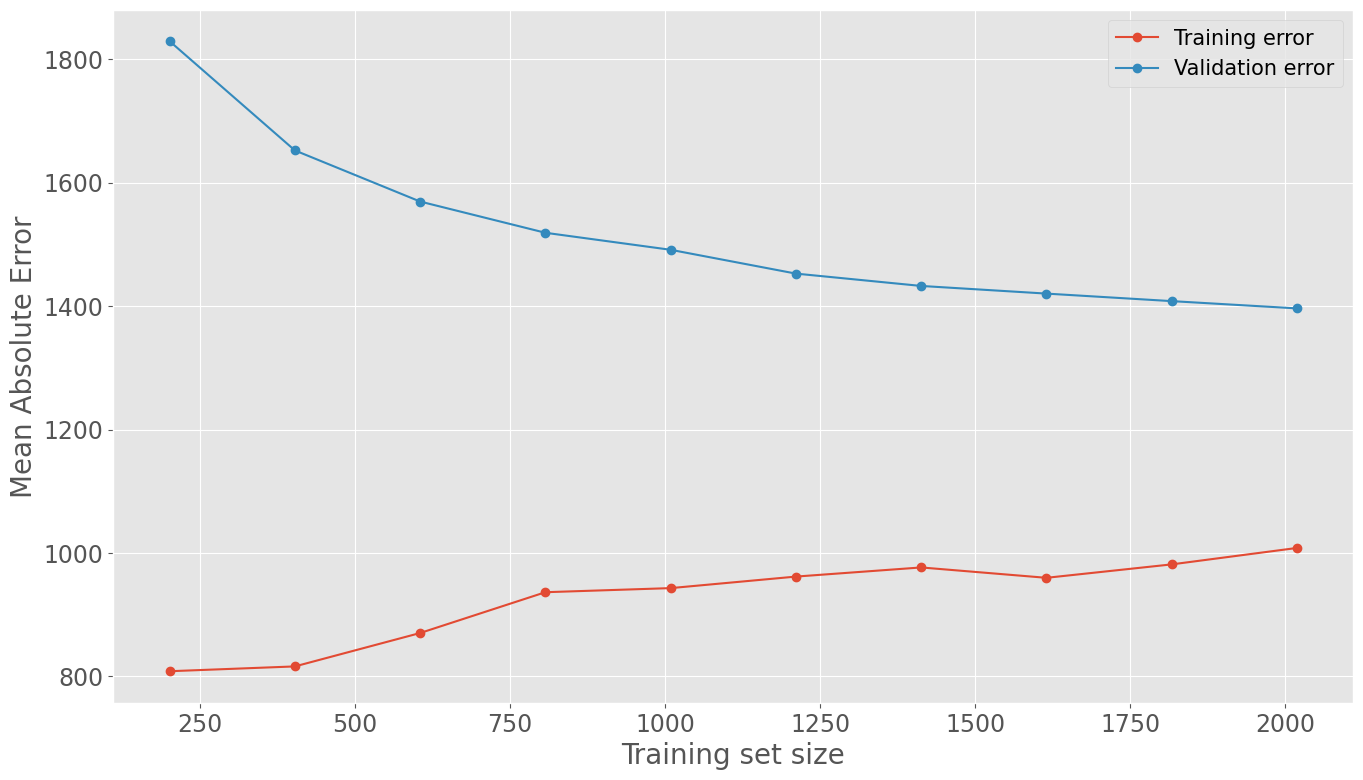
\includegraphics[width=0.7\textwidth]{"content/pics/Learning_curve.png"}
        \caption{Learning curve of the ensembled model for ten different sizes of the training subset.}
        \label{fig:learning_curve}
\end{figure}

The residuals (true minus predicted price) of the predicted and true prices for the ensembled model for the predicted prices are visualised in the scatter plot in \autoref{fig:Residuals_scatter_ensemble}.
\begin{figure}
    \centering
        \makebox[\textwidth][c]{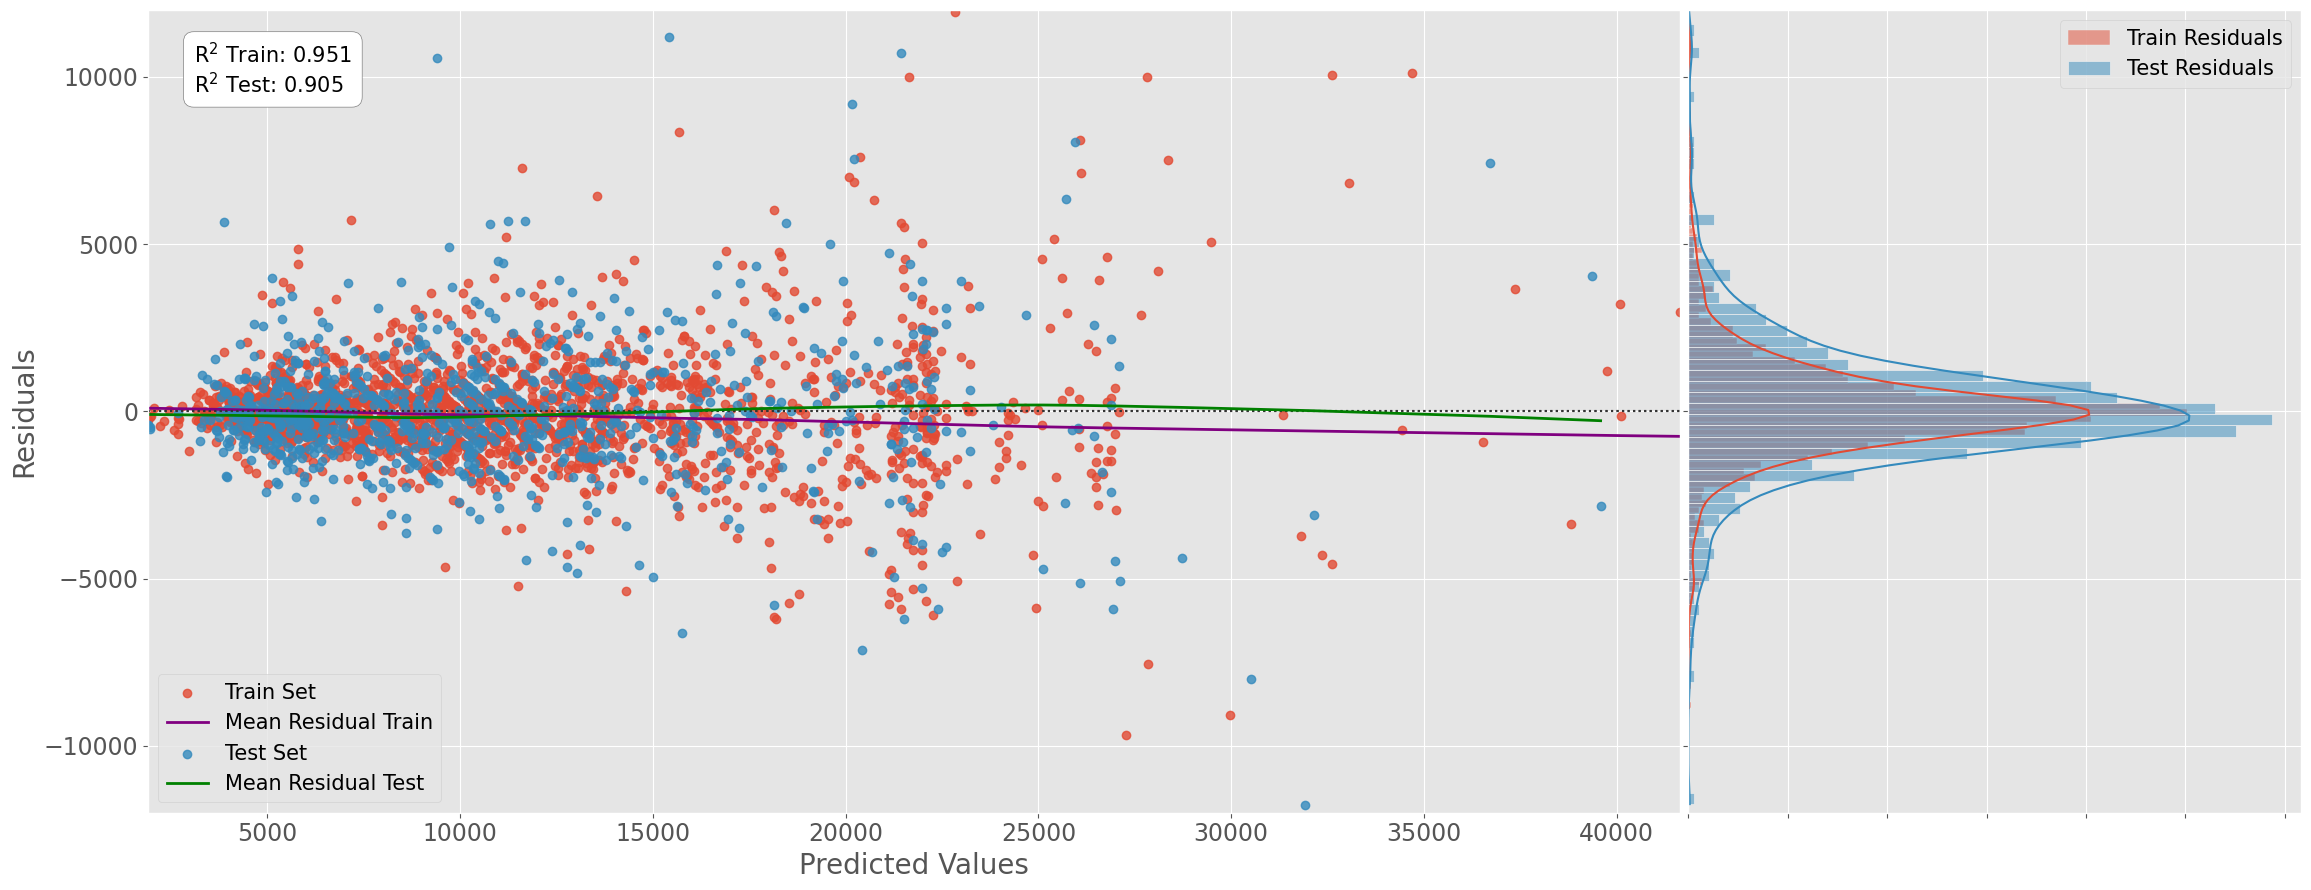
\includegraphics[width=1\textwidth]{"content/pics/residuals_train_test.png"}}
        \caption{Residuals for different predicted prices for the ensembled model for training and testing subsets. The model seems to overestimate the prices.}
        \label{fig:Residuals_scatter_ensemble}
\end{figure}

\autoref{fig:Tables} shows the data entries with the highest absolute residuals and therefore worst predictions. As suggested, these bikes are limited editions, which sell
for very high prices. An example of this is the first entry.

\begin{figure}
\centering
    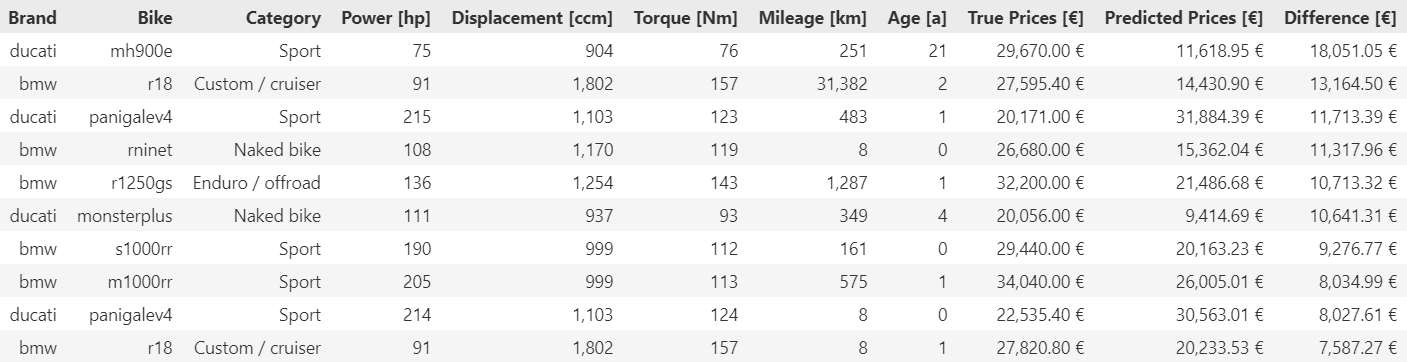
\includegraphics[width=\textwidth]{"content/pics/Table_Worst.png"}
\caption{Data entries with the highest residuals.}
\label{fig:Tables}
\end{figure}
Further plots for evaluation of the model are not included in this chapter to due a lack of space, but can be found in the \autoref{sec:Appendix}.